% -----------------------------------------------------------------------------
% Fundamentação Teórica
% -----------------------------------------------------------------------------

\chapter{Fundamentação Teórica}
\label{chap:fundamentacaoTeorica}

\section{Análise de dados em saúde}

A tomada de decisões em saúde precisa com frequência do suporte de um profissional especializado na temática a ser decidida. Uma série de técnicas são aplicadas por esse profissional para avaliação do contexto, uma vez que os dados puros não são suficientes, devido à multifatoriedade \cite{andrade_tomada_2008,resende2009}. O grande número de sistemas de auxílio em saúde, sejam esses de ordem regulatória ou ainda por iniciativas privadas, fazem com que o volume de dados cresça exponencialmente, produzindo o fenômeno de \emph{Big Data}. Uma definição conhecida desse conceito aponta volume, variedade e velocidade como os três vetores relacionados à produção massiva de dados \cite{laney20013d}. Outras características foram adicionadas a essa primeira definição de\emph{Big Data}, tais como veracidade \cite{schroeck2012analytics},  complexidade e desestruturação \cite{intel2012}, e valor \cite{oracle2013}.

A multifatoriedade já citada é um aspecto que se relaciona à complexidade dos dados em grande volumes. É cada vez mais difícil estabelecer uma relação de causa e efeito para a tomada de decisão segura, sem auxílio ou sumarização desses dados em informações mais tangíveis e associadas. Também é difícil descrever um algoritmo que permita analisar todos os dados de contexto e relacioná-los de forma que possa ser utilizado como substituição ao conhecimento tácito de um profissional da saúde experiente \cite{faceli2011}.

O suporte de sistemas, métodos e pŕaticas que auxiliem a assistência em saúde no tratamento de \emph{Big Data}  ainda não é suficientemente consolidado. Faltam evidências de aplicações especialmente quantitativas que validem seu uso nesse campo do conhecimento. Além disso, boa parte das tecnologias utilizadas nesses estudo estudos, utilizam recursos específicos de computação e frequentemente esses recursos têm custo elevado. Esses estudo focam na  avaliação de dados para otimização de recursos, suporte a decisões clínicas e redução de custo do cuidado \cite{nishita2018} e não na análise de dados para tomadas de decisão em saúde pública, nem tão pouco no auxílio para construção de politicas públicas. Ambos os focos são válidos, porém apresentam conceitos distintos e a forma de extrair essas informações são diferentes.

Há uma grande oportunidade de estudo na proposição de um \emph{stacks} (conjunto de ferramentas) e métodos para extrair essas informações no contexto de saúde pública. O desenvolvimento de abordagens para o processamento de dados nesse contexto de estudo pode viabilizar a utilização de grandes bases de dados públicas o que permitiria o estabelecimento de novas correlações e posteriormente associação com demais bancos, ou conjuntos de informações.

Sendo o paragrafo acima, justamente o que esse trabalho se propõe, ainda que o volume de dados da base sob análise neste trabalho e sua composição não qualifiquem como \emph{Big data}, sob a perspectiva de LANEY. Esse trabalho pode ser utilizado de base para uma nova forma de utilização de recursos computacionais na análise de grandes massas de dados e a posteriori \emph{Big Data}. 

\section{Virtualização}
Virtualização, no contexto de computação, é refere se à abstração de componentes e/ou recursos de computador. O objetivo do ambiente de computação virtual é melhorar a utilização de recursos, por meio da utilização sob demanda destes recursos, sendo essa demanda a forma de utilização e a quantidade de recursos necessários. Virtualização fornece uma plataforma operacional unificada e integrada para usuários e aplicativos com base na agregação de recursos heterogêneos e autônomos.

Essa abstração é, usualmente, feita por uma camada de software entre \emph{hardware} e SO (SO), chamada de \emph{hypervisor} ou monitor de maquina virtual (VMM).

Mais recentemente, a virtualização em todos os níveis (sistema, armazenamento e rede) tornou-se importante novamente como forma de melhorar a segurança, confiabilidade e disponibilidade do sistema, reduzir custos e fornecer maior flexibilidade.\cite{virt}

Existem diversos níveis de abstração para virtualização, considerando níveis mais detalhados de funcionalidades e/ou níveis menos específicos de hardware. Isso torna possível extrair aplicações e seus respectivos ambientes com mais facilidade e troca-los de máquina base, considerando essa mudança como portabilidade. Como objeto de estudo deste trabalho nos limitamos a definição de dois tipos de virtualização: completa, nível de SO.

\subsection{Virtualização completa}

Virtualização completa, sendo intermediada por sistema s VMM ou \emph{hypervisor} também é chamado de máquina virtual gerenciador e é executado em cima de um SO \emph{host}, geralmente como um aplicativo no SO base. O resultado é que, nas VMs, os aplicativos e o SO convidado são executados em cima de um hardware virtual fornecido pelo \emph{hypervisor}. Pode ser considerado para fornecer "Virtualização Completa".

Neste tipo de configuração, os dispositivos de E/S são atribuídos às máquinas convidadas (\emph{guest}), imitando os dispositivos físicos. A interação com esses dispositivos no ambiente virtual são então direcionados para os dispositivos físicos reais, seja pelo \emph{driver} do SO do host ou pelo "\emph{Driver VM}". 

Essa arquitetura pode ser observada na Figura \ref{fig:vms}. A principal vantagem dessa abordagem é que é muito fácil de usar. Um usuário comum pode instalar um produto de software como o \textregistered{VirtualBox} como qualquer outro produto de software no SO de sua escolha. Dentro do deste virtualizador, um SO \emph{guest} pode ser instalado e usado como se estivesse sendo executado diretamente no hardware. \cite{portnoy2012virtualization}

\begin{figure}[!h]
    \centering
    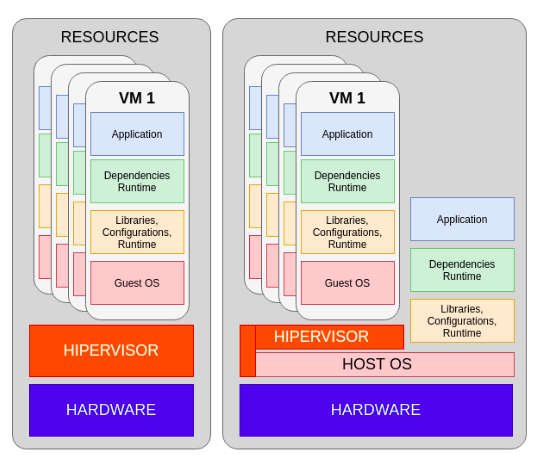
\includegraphics[width=0.8\textwidth]{04-figuras/vms.png}
    \caption{Hosted \emph{hypervisor} diagrama representativo de componentes (Fonte: Google Images, 2021)}
    \label{fig:vms}
\end{figure}

\subsection{Containers ou virtualização em nível de SO}

Conhecida também como \emph{container}, é uma técnica de virtualização que referece ao uso compartilhado do kernel do SO, porém manipula a forma de execução dos processo no \emph{userspace}, setando dois conjuntos de configurações, \emph{namespace} (isolamento dos recursos de sistema) e \emph{cgroup} (controle de utilização dos recursos).

\cite{redhat2018}
\subsubsection{Container}
\emph{Containers} são um conjunto de 1 ou mais processos sendo executados isolados do sistema base.

\subsubsection{Runtime}
Como no \emph{hypervisor} que executa e comunica com o sistema base ou hardware, para \emph{container} tempos o \emph{container} \emph{runtime} que é responsável por executar o \emph{container} e gerenciar o namespace e gcgroups definido para aquele \emph{container}.

\subsubsection{Orquestrator}
O orquestrador de \emph{container} é sistema responsável por avaliar e comandar a execussão dos \emph{container} por meio do \emph{runtime}, tendo como premissa a disponibilização dos recursos totais da maquina e garantindo que o \emph{container} esteja executando de acordo com uma  serie de parametros, bem como também é responsável pelas configurações de rede que serão utilizadas e gerenciadas ao logo do ciclo de vida dos \emph{container}s sob sua orquestração.

\section{Alternativas open source}

Para avaliar alternativas no mercado a seguinte estratégia de pesquisa foi conduzinda nas seguintes bases:

\begin{itemize}
    \item IEEE Xplore
    \item \emph{Computers and Applied Sciences Complete}
\end{itemize}

\subsection{Termos consultados}
Para organizar os termos selecionados para a busca, bem como a suas variações de consulta foi realizada uma agrupamento de palavras em temas e utilizadas combinações de termos de cada tema segundo a estrutura apresentada na tabela \ref{table:termos}.

A formatação da estratégia de pesquisa esta contida nas tabelas \ref{table:ieee} e \ref{table:computing}. Essa formatação permite indicar estudos que tenham os temas indicados de forma reduzida por assunto, título, palavras chave e resumo e a partir dessa extração, uma avaliação de ferramentas utilizadas resultou no levantamento de tecnologias a serem avaliadas na próxima sessão. Levando em consideração um filtro adicional que é ser \emph{Open Source}.

\begin{center}
\begin{table}[!htbp]
\begin{tabular}{cccc}
\textbf{CLUSTER}                                                  & \textbf{DATA PROCESSING}                                                                              & \textbf{COST}                                                                                                    & \textbf{COMPUTING}                                                                                                                               \\ \hline
\begin{tabular}[c]{@{}c@{}}cluster\\ “small cluster”\end{tabular} & \begin{tabular}[c]{@{}c@{}}“data process”\\ “data processing”\\ “data processing system”\end{tabular} & \begin{tabular}[c]{@{}c@{}}cost\\ “low cost”\\ “lowest cost”\\ “cheap”\\ “economic”\\ “inexpensive”\end{tabular} & \begin{tabular}[c]{@{}c@{}}computing\\ “grid computing”\\ “mist computing”\\ “cloud computing”\\ “fog computing”\\ “edge computing”\end{tabular} \\ \hline
\begin{tabular}[c]{@{}c@{}}\#1 Combinar \\ OR\end{tabular} & \begin{tabular}[c]{@{}c@{}}\#2 Combinar \\ OR\end{tabular} & \begin{tabular}[c]{@{}c@{}}\#4 Combinar \\ OR\end{tabular}                                                       & \#6 Combinar com OR \\ \hline
\multicolumn{1}{l}{} & \#3 \#1 AND \#2 & \#5 \#3 AND \#4 & \#7 \#5 AND \#6                                                                                                                                  \\ \hline
\end{tabular}
\caption{Termos de pesquisa e estratégia de agrupamento}
\label{table:termos}
\end{table}
\end{center}


\begin{table}[!htbp]
\centering
\begin{tabular}{ccc}
\textbf{Passo} & \multicolumn{1}{c}{\textbf{Operação}}                                                                                                                                               & \textbf{Resultados}  \\ \hline
\textbf{\#1}   & \begin{tabular}[c]{@{}l@{}}$$ALL = (\\ \ \ \ \ cluster\\ \ \ \ \ OR "small cluster"\\ )$$\end{tabular}  & 1.199.979  \\ \hline
\textbf{\#2}   & \begin{tabular}[c]{@{}l@{}}$$ALL = (\\ \ \ \ \ “data process” \\  \ \ \ \ OR “data processing” \\  \ \ \ \ OR “data processing system”\\ )$$\end{tabular} & 88.988  \\ \hline
\textbf{\#3}   & \#1 AND \#2 & 5.810  \\ \hline
\textbf{\#4}   & \begin{tabular}[c]{@{}l@{}}$$ALL = (\\  \ \ \ \ “low cost” \\  \ \ \ \ OR “lowest cost” \\  \ \ \ \ OR cheap \\  \ \ \ \ OR economic \\  \ \ \ \ OR inexpensive\\ )$$\end{tabular} & 1.836.782 \\ \hline
\textbf{\#5}   & \#3 AND \#4 & 206                 \\
\textbf{\#6}   & \begin{tabular}[c]{@{}l@{}}$$ALL = (\\  \ \ \ \ “grid computing” \\  \ \ \ \ OR “mist computing”  \\  \ \ \ \ OR “cloud computing”\\  \ \ \ \ OR “fog computing”\\  \ \ \ \ OR “edge computing”\\ )$$\end{tabular} & 81.679 \\ \hline
\textbf{\#7}   & \#5 AND \#6 & 22   
\end{tabular}
\caption{Estratégia de pesquisa em IEEE}
\label{table:ieee}
\end{table}

\begin{table}[!htbp]
\centering
\begin{tabular}{ccc}
\textbf{Passo} & \textbf{Operação}                                                                                                                                                & \textbf{Resultados} \\ \hline
\textbf{\#1}   & \begin{tabular}[c]{@{}l@{}}TITLE-ABS-KEY (\\  \ \ \ \   cluster \\  \ \ \ \  OR "small cluster"\\  \ \ \ \   )\end{tabular} & 963.442 \\ \hline
\textbf{\#2}   & \begin{tabular}[c]{@{}l@{}}TITLE-ABS-KEY  (\\  \ \ \ \   "data process" \\  \ \ \ \   OR "data processing" \\  \ \ \ \   OR "data processing system" \\   \ \ \ \  )\end{tabular} & 316.839 \\ \hline
\textbf{\#3}   & \#1 AND \#2 & 8.190 \\ \hline
\textbf{\#4}   & \begin{tabular}[c]{@{}l@{}}TITLE-ABS-KEY  (\\  \ \ \ \   "low cost"\\  \ \ \ \   OR "lowest cost"\\  \ \ \ \   OR cheap\\  \ \ \ \   OR economic\\  \ \ \ \   OR inexpensive\\  \ \ \ \   )\end{tabular} & 2.294.081 \\ \hline
\textbf{\#5}   & \#3 AND \#4 & 347 \\ \hline
\textbf{\#6}   & \begin{tabular}[c]{@{}l@{}}$$ALL = (\\ “grid computing” \\  \ \ \ \  OR “mist computing” \\  \ \ \ \  OR “cloud computing” \\  \ \ \ \  OR “fog computing” \\  \ \ \ \  OR “edge computing”\\ )$$\end{tabular} & 125.105 \\ \hline
\textbf{\#7}   & \#5 AND \#6 
\end{tabular}
\caption{Estratégia de pesquisa em \emph{Computers and Applied Sciences Complete}}
\label{table:computing}  
\end{table}

\subsection{Seleção de tecnologias}

Com a pesquisa descrita acima, pudemos filtrar tecnologias e ferramentas de mercado utilizadas em clusters de baixo custo e como estratégias para a análise de dados, o que retornou um grande número de artigos.  Para fins de apresentação dessas soluções neste trabalho, elas foram agrupadas conforme níveis de complexidade de implementação, sempre mantendo o custo como restrição primária e o contexto de aplicação sendo para instituições com grande restrição orçamentária.
Diante disso, e tendo em vista o tamanho da base de dados de origem, durante o levantamento de material para o projeto foram avaliadas soluções em dois grupos:

\begin{itemize}
    \item Computação em nuvem privada; e
    \item Orquestração de \emph{Containers}.
\end{itemize}



Na primeira categoria, a utilização de ferramentas como \emph{OpenStack}\textregistered e \emph{CloudStack}\textregistered foram consideradas. No entanto, observa-se que nesse tipo de utilização existe um \emph{overhead} substancial, tanto em termos de complexidade de configuração, quanto em termos de hardware necessário para operar de maneira eficiente. Essas alternativas requerem maior capacidade computacional, conforme suas configurações recomendadas \cite{cloudstack,openstack}. Além disso, as soluções de nuvem privada estendem muito o propósito de orquestração de cargas de trabalho, provendo todo o conceito de infraestrutura como serviço (Iaas). E, dependendo da implementação e dos componentes utilizados, elas provêm plataforma como serviço (PaaS), que são categorias de abstração do hardware, configurações e sistemas de suporte/apoio como sistema operacional (SO) para aplicação \cite{openstack,cloudstack,mell_nist_2011}. Logo, embora sejam alternativas populares, tornam o processo substancialmente mais complexo e, portanto, foram descartadas para essa avaliação, tendo em vista o escopo deste trabalho.

Na segunda categoria, sistemas de orquestração de \emph{container}s possuem um baixo \emph{overhead} devido à arquitetura do \emph{container} (Figura \ref{fig:container}), compartilhando parte do kernel space. Logo, não necessita de uma camada de virtualização do SO, presente em virtualizações completas e gerenciadas por \emph{hypervisors} (Figura )\ref{fig:vmscontainer}). Vale ressaltar que essa solução oferece ainda algumas possibilidades como, por exemplo,  o gerenciamento de capacidade dos nós do \emph{cluster} para agendamento de tarefas. Dentre as plataformas disponíveis, o Kubernetes\textregistered é apontado como uma das principais soluções de orquestração de \emph{container}s, tanto pela disponibilidade de features, quando pelos projetos em operação e pelo tamanho de sua comunidade \cite{truyen_comprehensive_2021}. O Kubernetes\textregistered tem o apoio de entidades como Cloud Native Computing Foundation (CNCF), que apoiam e supervisionam a plataforma de software -  definida como peça importante de software, sob o qual diversos programas de aplicativos menores podem ser projetados para serem executados \cite{collins2022}. Esse apoio tem como objetivo a expansão  das capacidades, endereçando problemas conhecidos e situações de uso, bem como estabelecendo padrões para tecnologias que pertencem ao ecossistema de orquestração de \emph{container}s.

\begin{figure}[!h]
    \centering
    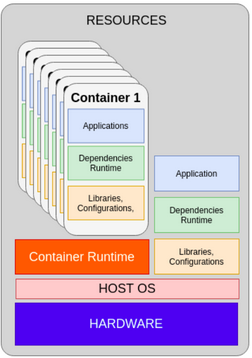
\includegraphics[width=0.3\textwidth]{04-figuras/containers.png}
    \caption{Estrutura do \emph{container} (elaborada pelo autor)}
    \label{fig:container}
\end{figure}

\begin{figure}[!h]
    \centering
    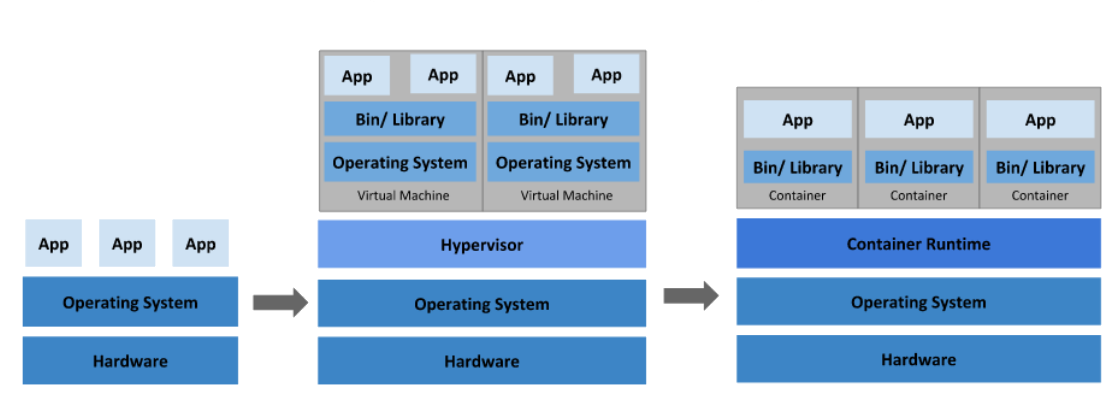
\includegraphics[width=0.8\textwidth]{04-figuras/vmsContainer.png}
    \caption{Eras de \emph{deployment}s e sua evolução por tecnologia base (Fonte: The Linux Foundation\textregistered, 2021)}
    \label{fig:vmscontainer}
\end{figure}

Soluções como Apache Mesos, Hashicorp Nomad, e Docker Swarm também foram avaliadas pelo estudo de \cite{truyen_comprehensive_2021}, mas em todos os casos foram citadas diferenças significativas, especialmente no uso, sendo o Kubernetes\textregistered a melhor por eles avaliada. 

\section{Cluster orquestrador de \emph{container}}

Kubernetes\textregistered é a consolidação de quinze anos de trabalho da Google\textregistered com orquestração de cargas de trabalho, processamentos \emph{batch}, e um sistema interno de gerenciamento de \emph{cluster} orientado a \emph{container}s, o Borg \cite{verma_large-scale_2015}. 

As estruturas básicas do Kubernetes\textregistered são divididas em componentes com atribuições bem definidas, como na Figura \ref{fig:kubenode}. Os componentes que são essenciais à proposta deste trabalho são:
\begin{itemize}
    \item \emph{Kube-apiserver}, que concentra toda a api do kubernetes
    \item \emph{Kube-scheduler}, que avalia novos pods e em qual nó worker do \emph{cluster} eles serão alocados
    \item \emph{Kube-controller-manager}, que comporta os objetos de controle do kubernetes
    \item \emph{Kubelet}, responsável por repassar comando do control plane, para o worker e comunicar com \emph{container} \emph{runtime}
    \item \emph{Kube-proxy}, responsável por toda a estrutura de redes nativa do kubernetes e pods do \emph{cluster}
    \item \emph{Pod}, menor unidade de \emph{deployment}, podendo conter um conjunto de \emph{container}s que compõem uma solução.
\end{itemize}

\begin{figure}[!h]
    \centering
    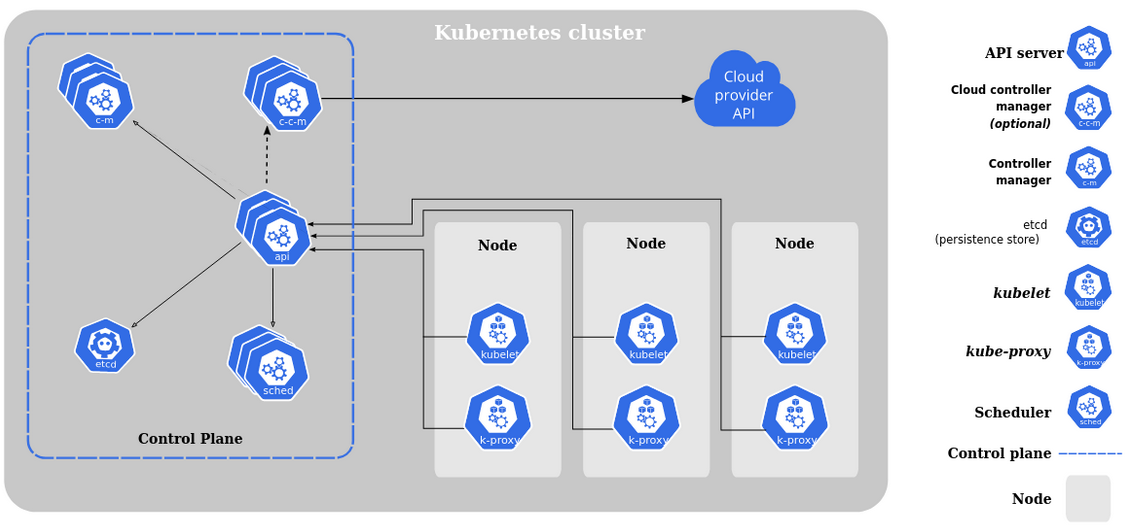
\includegraphics[width=0.8\textwidth]{04-figuras/kubeadm-node.png}
    \caption{Kubernetes arquitetura de componentes (Fonte: The Linux Foundation\textregistered, 2021)}
    \label{fig:kubenode}
\end{figure}



